\chapter{Identification of individual treatment effects by imputing potential outcomes with partial correlation specification} 
\label{chap4}
	\begin{abstract}
		In most medical research, the treatment effect is calculated by the average treatment effect. However, precision medicine requires knowledge of individual treatment effects, which is how individuals respond to treatment. Because only one potential outcome is observed for each unit, the causal inference is a missing data problem. We proposed a multiple imputation approach to assess individual treatment effects, which allows the researcher to consider the heterogeneity of treatment effects unexplained by observed variables. The method needs to specify the partial correlation between potential outcomes since there is no relevant information in the observed data. Therefore, it is helpful to perform sensitivity analysis on the partial correlation. We showed that our approach provides valid inference of marginal distribution of potential outcomes. However, the posterior distribution of individual treatment effects varies with different specified partial correlations. According to the various posterior distribution of individual treatment effects, the researcher would comprehensively understand optimal treatment recommendations. We also apply our method to an HIV study and discuss further research directions.
	\end{abstract}
	
	\section{Introduction}
	\label{sec:4.1}
	Heterogeneity of treatment effects (HTE) across individuals is an essential complication in precision treatment assignment to different persons. Attention to variability in treatment effects is increasing. If the true effect varies across individuals, the average treatment effect (ATE) leads to suboptimal individual treatment recommendations. The usual approach to assess HTE is subgroup analyses based on observed effect modifiers \citep{poulson2012treatment, zhang2013assessing}. A subgroup analysis explains the HTE by observed data in different subpopulations. In fact, if all variables relevant to the heterogeneous treatment effect are available, we can build a model to estimate outcomes under all treatment levels. However, in practice, we rarely have all effect modifiers known and collected. In that case, there would be a fraction of HTE that cannot be explained by observed data, a situation known as idiosyncratic variation \citep{ding2016randomization, heckman1997making} or residual HTE \citep{zhang2013assessing}.
	
	In HTE, treatment effects vary by individual. The individual treatment effect (ITE) is the basic element in causal inference. We can always estimate average treatment effects, HTE or other statistics of interest from individual treatment effects. The potential outcomes framework stipulates that each individual has a potential outcome under each possible treatment level. \citet{ding2018causal} reviewed various methods of estimating potential outcomes. 
	
	The difficulty of evaluating ITE from the observed data is that only one of the treatment outcomes is observed for each individual \citep{rubin1974estimating, hernan2010causal}. This fundamental problem of causal inference implies that causal inference is essentially a missing data problem \citep{rubin2005causal, ding2018causal}. In this paper, we study the use of multiple imputation to quantify unobserved outcomes. In multiple imputation, each missing value is filled in multiple times to reflect the uncertainty about the true but unobserved value. After imputing missing values in potential outcomes, we can estimate the individual treatment effect on the completed datasets. 
	
	\citet{lamont2018identification}, and \citet{westreich2015imputation} discuss previous work on multiple imputation and potential outcomes. These authors fit the imputation model for a potential outcome based on observed pre-treatment variables, which we call multiple marginal imputation (MMI). MMI assumes conditional independence between potential outcomes. This assumption cannot be verified from the observed data \citep{rassler2012statistical}. \citet{imbens2015causal} and \citet{gadbury2001evaluating} elucidate sensitivity of the estimates under violations of the assumption. \citet{Buuren2018} demonstrated that if one imputes the unobserved outcomes using only the observed outcome as a predictor, the derived imputed outcomes are unstable and implausible. \citet{smink2016towards} proposed a data augmentation approach to specify the correlation between potential outcomes. Smink focused on the situation without any covariates. With a proper prior specification of the joint distribution of potential outcomes, additional concatenated cases are generated and included in the observed data. In that case, the correlation between the imputed dataset's potential outcomes is close to the specified value and, hence, the imputed dataset is stable. However, it becomes challenging to specify the prior joint distribution for the augmented data if there are covariates. Proposed approaches for estimating potential outcomes are diverse. One of them is the targeted learning method, which is a machine learning based approach. It first fits the data-generating process among a set of reasonable models and then reduces the bias in estimating the parameter of interest iteratively. When evaluating the potential outcomes, the scientific interest is usually the average treatment effect.   
	
	This paper explores a new block imputation approach for missing potential outcomes with covariates. To clarify ideas, we focus on continuous outcomes. Potential outcomes are assumed with a multivariate normal distribution and imputed in one block. We introduce the notation, describe the potential outcomes framework and explore the role of the partial correlation between potential outcomes in causal inference in section \ref{sec:4.2}. Section \ref{sec:4.3} provides an overview of the joint modeling method (JM) and the fully conditional specification method (FCS) and introduces block imputation, a hybrid of JM and FCS. We describe our proposed method, which imputes missing potential outcomes with partial correlation specification in section \ref{sec:4.4}. To assess the validity of our method, we perform simulation studies and comparisons with the targeted learning in section \ref{sec:4.5}. Section \ref{sec:4.6} demonstrates the applicability of our proposed approach in a clinical trial that aimed to compare the effect of four different therapies on slowing the progression of HIV disease. In section \ref{sec:4.7}, we conclude with a discussion. 
	
	\section{Framework}
	\label{sec:4.2}
	\subsection{Notation}
	Let ${Y(j), j = 1, \dots, p}$ denote one of $p$ incomplete variables and $Y(-j) = (Y(1), \dots, Y(j-1), Y(j+1),\\ \dots, Y(p))$ denote the collection of the $p-1$ variables in $Y$ except $Y(j)$. In this paper, $Y(j)$ ususally represents the potential outcomes. Let $X = (X(1), \dots, X(k))$ be a set of $k$ completely observed variables. Let $\rho(Y(0), Y(1))$ be the correlation between two potential outcomes and $\rho_{Y(0), Y(1)\,|\ X}$ be the partial correlation between two potential outcomes. 
	\subsection{Setup}  
	We focus on the case of a binary treatment $W_{i}$ and a continuous outcome $Y_{i}$ and assume the data come from a random sample of individuals, indexed by $i \in {1,\cdots,N}$. Each individual $i$ has a nonzero probability to be assigned to both treatments, with $W_{i} = 1$ for the active treatment and $W_{i} = 0$ for the control treatment. The number of units under treatment and control are $N_{1}$ and $N_{0}$ respectively. We assume that the treatment assignment mechanism is unconfounded by the unobserved outcomes $Y_{mis}$, i.e., an ignorable assignment mechanism. We also assume that the potential outcomes for any individual are independent of the treatments assigned to others, which is known as the Stable Unit Treatment Value Assumption \citep{imbens2015causal}. Here the ignorable or unconfounded assignment mechanism implies that $P(W|Y(0), Y(1), X) = P(W|Y_{obs}, X)$, where X are observed covariates not influenced by treatment assignment. The individual treatment effect is defined as $\tau_{i} = Y_{i}(1) - Y_{i}(0)$. We assume a joint distribution for the potential outcomes $Y_{1}$ and $Y_{0}$ and that the correlation between the potential outcomes $\rho(Y_{1}, Y_{0})$ can be quantified by one or more parameters. The imputation models for missing outcomes $Y(1)$ and $Y(0)$ are: 
	\begin{align}
		\dot{Y}(1) &\sim P(Y^{mis}(1)|Y^{obs}(1), Y(0), X, \dot{\phi}_{1})\\
		\dot{Y}(0) &\sim P(Y^{mis}(0)|Y^{obs}(0), Y(1), X, \dot{\phi}_{0}),
	\end{align}
	where parameters of the imputation model $\dot{\phi}_{1}$ and $\dot{\phi}_{0}$ are draws from their respective posterior distribution.
	\subsection{Partial correlation between potential outcomes}
	We decompose the individual treatment effect $\tau_{i} \in T, i = 1, \dots, N$ via
	\begin{equation}
		\begin{array}{lr}
			\tau_{i} = Y_{i}(1) - Y_{i}(0) = X_{i}^{T}\beta + \epsilon_{i},
		\end{array}
	\end{equation}
	where $X_{i}$ are observed pre-treatment covariates for individual $i$. Under random treatment assignment, the regression weight $\beta$ could be the ordinary least-square (OLS) estimation of $\tau_{i}$ on $X_{i}$. The quantity $X_{i}^{T}\beta$ is known as systematic treatment effect variation and the residual $\epsilon_{i}$ is the idiosyncratic treatment effect variation not explained by $X_{i}$ \citep{ding2019decomposing, heckman1997making, djebbari2008heterogeneous}. The idiosyncratic variation accounts for treatment effect variation not attributable to differences in observed covariates. Based on the formula of OLS estimation, the coefficient 
	\begin{equation}
		\begin{array}{cl}
			\beta &= (X^{T}X)^{-1}X^{T}T \\
			&= (X^{T}X)^{-1}X^{T}Y(1) - (X^{T}X)^{-1}X^{T}Y(0) \\
			&= \beta_{1} -\beta_{0},
		\end{array}
	\end{equation}
	where $\beta_{1}$ and $\beta_{0}$ are the corresponding regression weights of the potential outcomes $Y_{1}$ and $Y_{0}$ on the observed covariates $X$. Similarly, the idiosyncratic treatment effect variation $\epsilon_{i}$
	\begin{equation}
		\begin{array}{cl}
			\epsilon_{i} &= \tau_{i} - X_{i}^{T}\beta\\
			&= (Y_{i}(1)  - X_{i}^{T}\beta_{1}) - (Y_{i}(0) - X_{i}^{T}\beta_{0})\\
			&= \epsilon_{i}(1) -\epsilon_{i}(0),
		\end{array}
	\end{equation} 
	where $\epsilon(1)$ and $\epsilon(0)$ are the residuals from the regression of the potential outcomes $Y_{1}$ and $Y_{0}$ on the observed covariates $X$. Applying the theory of variance decomposition for linear regression, we could decompose the variance of individual treatment effect into two components:
	\begin{equation}
		var(\tau_{i}) = var(X_{i}^{T}\beta) + var(\epsilon_{i}). 
	\end{equation}
	Based on the idiosyncratic treatment effect variation formula (5), the idiosyncratic components of individual treatment variance becomes
	\begin{equation}
		\begin{array}{cl}
			var(\epsilon_{i}) &= var(\epsilon_{i}(1) -\epsilon_{i}(0))\\ 
			&= var(\epsilon_{i}(1)) + var(\epsilon_{i}(0)) - 2cov(\epsilon_{i}(1), \epsilon_{i}(0)), 
		\end{array}
	\end{equation} 
	which demonstrate that partial correlation between potential outcomes $\rho_{Y(0)Y(1)\,|\ X}$ does impact the idiosyncratic variation which is unidentifiable from the observed data. 
	
	We provide three approaches to identify the partial correlation between potential outcomes: the model-based approach, the experiment-based approach, and sensitivity analysis. The model-based approach explicitly models the relationship between the idiosyncratic variation and the assignment mechanisms such that the partial correlation would be close or equal to zero \citep{heckman2005scientific}. Economists usually deal with ex-post causal inference. The agents select the treatment according to their ex-ante evaluation. In this case, economists could infer the information only available to agents from the assignment mechanism.  For instance, \citet{heckman2010effects} investigated the causal effect of educational decisions on the labor market and health outcomes. He modeled latent cognitive and social-emotional endowments and included these latent variables into the outcome equations. As indicated earlier, the partial correlation between potential outcomes is the only unknown parameter in the formula of idiosyncratic variation. The model for idiosyncratic variation could be tailored to the model for the partial correlation between potential outcomes. Generally, the model-based approach attempts to figure out latent variables affecting the partial correlation between potential outcomes. 
	
	The experiment-based approach intends to design sophisticated experiments to collect additional data where analysts could evaluate the partial correlation between potential outcomes. For instance, the experiment-based approach collects repeated measurements under more than one treatment level for the same individual from which some relevant information about the partial correlation between potential outcomes is available. The experiment designed for repeat measurements is known as N-1 trails \citep{shamseer2015consort, araujo2016understanding}. Researchers could also design an auxiliary treatment ($W_{i} = 2$) and assignment the extensive treatment to all individuals in the sample. Then the individual treatment effect $Y_{i}(1) - Y_{i}(0)$ can be evaluated by $(Y_{i}(2) - Y_{i}(0) - (Y_{i}(2) - Y_{i}(1))$. 
	
	Both model-based and experiment-based approaches search for extra information to determine the partial correlation between potential outcomes. If such additional information is not available, the alternative is sensitivity analysis. One could impute the missing potential outcomes and evaluate individual treatment effects with various valid partial correlations and study the effect on the conclusions \citep{gadbury2001evaluating}. 
	
	\section{Methodology}
	\label{sec:4.3}
	\subsection{Joint modeling imputation (JM)}
	Joint modeling imputation assumes a model $p(Y^{mis}, Y^{obs}\,|\,\theta)$ for the complete data and a prior distribution $p(\theta)$ for the parameter $\theta$. Joint modeling partitions the observed data into groups based on the missing pattern and imputes the missing data within each missing pattern according to corresponding predictive distribution. Under the assumption of ignorability, the parameters of the predictive distribution for different missing patterns are generated from the posterior joint distribution. \citet{schafer1997analysis} proposed joint modeling methods for multivariate normal data, categorical data and mixed normal-categorical data. The joint modeling approach has solid theoretical properties (i.e., compatibility between the imputation and substantive models) while it lacks the flexibility of model specification.
	
	\subsection{Fully Conditional Specification (FCS)}
	In Fully Conditional Specification, we specify the distribution for each partially observed variable conditional on all other variables $P(Y(j)|Y(-j), X, \theta_{j})$ and impute each missing variable iteratively. The FCS starts with naive imputations such as a random draw from the observed values. The \emph{t}th iteration for the incomplete variable \emph{$Y(j)$} consists of the following draws:
	\begin{align*}
		&\theta_{j}^{t} \sim f(\theta_{j})f(Y^{obs}(j)|Y^{t-1}(-j), X, \theta_{j})\\
		&Y^{mis(t)}(j) \sim f(Y^{mis}(j)|Y^{t}(-j), X, \theta_{j}^{t}),
	\end{align*}
	where $f(\theta_{j})$ is generally specified as a noninformative prior. After a sufficient number of iteration, typically with 5 to 10 iterations \citep{Buuren2018, oberman2020missing}, the stationary distribution is achieved. The final iteration generates a single imputed dataset and the multiple imputations are created by applying FCS in parallel \emph{m} times. Since FCS provides tremendous flexibility in specifying imputation models for multivariate partially observed data, FCS is now a widely accepted and popular MI approach \citep{van2007multiple}. Even while, FCS lacks a satisfactory theory and has a potential risk in incompatibility. 
	
	\subsection{Block imputation}
	Block imputation combines the flexibility of FCS with the attractive theoretical properties of JM. A block consists of one or more variables. If the block has multiple variables, then we use multivariate imputation methods to impute those variables jointly. A simple example would be multiple imputation of missing variables with quadratic effects $Y = \alpha + \beta_{1}X + \beta_{2}X^2 + \epsilon$. In such a case, grouping the missing variable $X$ and its corresponding square term $X^2$ within one block is of benefit to preserve the quadratic relationship \citep{vink2019}. The joint modeling approach is the special case where all variables form one block, while the FCS approach treats each variable as a separate block. 
	
	When the imputation model of one variable is potentially incompatible, or its theoretical properties are not fully studied (i.e., whether the imputations based on the FCS correspond to drawing from a joint distribution), block imputation would merge that variable with other variables and apply the joint modeling imputation approach to that block. On the other hand, when the joint distribution of several missing variables is ambiguous, block imputation could use the FCS approach to impute each variable. In general, the apparent advantage of block imputation is the flexibility of model specification. However, block methods are hardly known or studied. While available in the \texttt{mice} software, the properties of block imputation have yet to be studied. 
	
	\section{BLI-SPC}
	\label{sec:4.4}
	This section describes how the block imputation could be used to impute missing outcomes with a given partial correlation between potential outcomes. We term the algorithm the block imputation algorithm with specified partial correlation (BLI-SPC). Since the missing pattern of potential outcomes is somehow restrictive, that is, no cases with completely observed potential outcomes, the imputation procedure is comprised of three steps. The first step involves estimating the marginal distribution of potential outcomes conditioning on pre-treatment variables. The second step consists of deriving the multivariate density of potential outcomes by combining the marginal distribution of potential outcomes and the specified correlation between potential outcomes. The third step imputes the missing outcomes with the corresponding submodel obtained from the multivariate distribution. 
	
	Our approach shares some similarities with statistical matching discussed by \citet{moriarity2003note}. Suppose there are two sample files, A and B. File A collects variables $X$ and $Y$ and file B collects variables $X$ and $Z$. The purpose of statistical matching is to combine two files, A and B, into one file containing variables $X$, $Y$ and $Z$. \citet{rubin1986statistical} proposed a procedure of statistical matching with three steps: regression step, matching step and concatenation step. In the regression step, Rubin specified the correlation between variable $X$ and $Y$ to derive the joint distribution of ($X$, $Y$, $Z$) in two sample files. We develop this idea to evaluate the individual treatment effects and extend to multiple treatments condition.  
	  
	
	Without loss of generality, let us assume that potential outcomes follow a multivariate normal distribution. We specify Bayesian linear models for two potential outcomes based on observed covariates. 
	\begin{align}
		Y(0) = \beta_{0}X + \epsilon_{0}, \epsilon_{0} \sim \mathcal{N}(0, \sigma_{0}^2)\\
		Y(1) = \beta_{1}X + \epsilon_{1}, \epsilon_{1} \sim \mathcal{N}(0, \sigma_{1}^2)
	\end{align}
	Bayesian sampling draws $\beta_{0}^{*}$, $\beta_{1}^{*}$, $\sigma_{0}^{*2}$, $\sigma_{1}^{*2}$ from their respective posterior distribution. The Jeffrey's prior used and hence, the posterior distributions of $\sigma_{0}^{*2}$ and $\sigma_{1}^{*2}$ would be inverse $\chi^2$ distribution:
	\begin{align}
		\sigma_{0}^{*2} \sim \sum_{i = 1}^{N_{0}}(Y_i(0) - \hat{\beta}_{0}X_{i})^2\chi_{N_{0} - k}^{-2}\\
		\sigma_{1}^{*2} \sim \sum_{i = 1}^{N_{1}}(Y_i(1) - \hat{\beta}_{1}X_{i})^2\chi_{N_{1} - k}^{-2}
	\end{align}
	where $\hat{\beta}_{0} = (X_{0}'X_{0})^{-1}X_{0}'Y(0)$, $\hat{\beta}_{1} = (X_{1}'X_{1})^{-1}X_{1}'Y(1)$ and \emph{k} is the number of covariates. The conditional distributions of  $\beta_{0}^{*}$ and $\beta_{1}^{*}$ are multivariate normal:
	\begin{align}
		\beta_{0}^{*} | \sigma_{0}^{*2} \sim \mathcal{N}(\hat{\beta}_{0}, \sigma_{0}^{*2}((X_{0}'X_{0})^{-1}))\\
		\beta_{1}^{*} | \sigma_{1}^{*2} \sim \mathcal{N}(\hat{\beta}_{1}, \sigma_{1}^{*2}((X_{1}'X_{1})^{-1}))
	\end{align}
	Since there is no information relevant to the partial correlation between potential outcomes in the observed data, the posterior distribution of the partial correlation $\rho_{Y(0)Y(1)|X}$ equals the prior distribution specified by the user, who can select several numbers in the interval [$-1$, $1$] to investigate the sensitivity to $\rho_{Y(0)Y(1)|X}$. 
	Finally, combined the marginal distribution of $Y(0)$ and $Y(1)$ with the specification of $\rho_{Y(0)Y(1)|X}$, the joint distribution of $Y^{mis}(0)$ and $Y^{mis}(1)$ is:
	\begin{eqnarray}
		\left[\begin{array}{c}
			Y^{mis}(0)\\
			Y^{mis}(1)
		\end{array}\right] & \sim & \mathcal{N}\left[\left(\begin{array}{c}
			\beta^{*}_{0}x\\
			\beta^{*}_{1}x
		\end{array}\right),\left(\begin{array}{cc}
			\sigma^{*2}_{0} & \rho_{Y(0)Y(1)|X}\sigma^{*}_{0}\sigma^{*}_{1}\\
			\rho_{Y(0)Y(1)|X}\sigma^{*}_{0}\sigma^{*}_{1} & \sigma^{*2}_{1} 
		\end{array}\right)\right]
	\end{eqnarray}
	and the distributions of $Y^{mis}(0)$ and $Y^{mis}(1)$ are:
	\begin{align}
		Y^{mis}(0) \sim \mathcal{N} (\beta^{*}_{0}x + (Y(1) - \beta^{*}_{1}x)\rho_{Y(0)Y(1)|X}\sigma_{0} / \sigma_{1}, (1 - \rho_{Y(0)Y(1)|X}^2)\sigma^{*2}_{0})\\
		Y^{mis}(1) \sim \mathcal{N} (\beta^{*}_{1}x + (Y(0) - \beta^{*}_{0}x)\rho_{Y(0)Y(1)|X}\sigma_{1} / \sigma_{0}, (1 - \rho_{Y(0)Y(1)|X}^2)\sigma^{*2}_{1})
	\end{align}
	Comparing equations (15) and (16) to equations (8) and (9), it is evident that inclusion of the observed outcome may change the location of missing outcomes shifts slightly and the uncertainty is reduced when imputing missing outcomes under the specified correlation between potential outcomes. For the prediction of units out of trials, the reasonable values for outcomes under two treatments could be drawn from the joint distribution (14). 
	
	When generalizing to the multiple treatments condition $W = 0, 1,\dots,w$, the marginal posterior distribution for potential outcomes would be:
	\begin{align*}
		Y(0)^{*} &= \beta_{0}^{*}X + \epsilon_{0}^{*}, \epsilon_{0}^{*} \sim \mathcal{N}(0, \sigma_{0}^{*2})\\
		Y(1)^{*} &= \beta_{1}^{*}X + \epsilon_{1}^{*}, \epsilon_{1}^{*} \sim \mathcal{N}(0, \sigma_{1}^{*2})\\
		&\dots\\
		Y(w)^{*} &= \beta_{w}^{*}X + \epsilon_{w}^{*}, \epsilon_{w}^{*} \sim \mathcal{N}(0, \sigma_{w}^{*2})
	\end{align*}
	where the values of $\beta_{0}^{*}$, $\beta_{1}^{*}$, \dots, $\beta_{w}^{*}$, $\sigma_{0}^{*2}$, $\sigma_{1}^{*2}$, \dots, $\sigma_{w}^{*2}$  draw from their respective Bayesian posterior distribution.
	If $\sigma_{0}^{*2}, \dots, \sigma_{w}^{*2}$ are unrestricted, with pairwise specification of partial correlation between potential outcomes, the joint distribution of $Y^{mis}(0)$, $Y^{mis}(1)$, \dots, $Y^{mis}(w)$ is:
	\begin{eqnarray}
		\left[\begin{array}{c}
			Y^{mis}(0)\\
			Y^{mis}(1)\\
			\dots\\
			Y^{mis}(w)
		\end{array}\right] & \sim & \mathcal{N}\left[\begin{array}{c}
			\mathcal{M}
		\end{array},\begin{array}{c}
			\Sigma\\
		\end{array}\right],
	\end{eqnarray}
	where  $\mathcal{M} = (\beta^{*}_{0}x, \beta^{*}_{1}x, \dots, \beta^{*}_{w}x)^T$. The covariance matrix $\Sigma$ must be positive semi-definite:
	\begin{eqnarray}
		\begin{array}{c}
			\Sigma
		\end{array} = \left(\begin{array}{cccc}
			\sigma^{*2}_{0} & \rho_{Y(0)Y(1)|X}\sigma^{*}_{0}\sigma^{*}_{1} & \dots & \rho_{Y(0)Y(w)|X}\sigma^{*}_{0}\sigma^{*}_{w}\\
			\rho_{Y(1)Y(0)|X}\sigma^{*}_{1}\sigma^{*}_{0} & \sigma^{*2}_{1} & \dots & \rho_{Y(1)Y(w)|X}\sigma^{*}_{1}\sigma^{*}_{w}\\
			\vdots & \vdots & \ddots & \vdots\\
			\rho_{Y(w)Y(0)|X}\sigma^{*}_{w}\sigma^{*}_{0} & \rho_{Y(w)Y(1)|X}\sigma^{*}_{w}\sigma^{*}_{1} & \dots & \sigma^{*2}_{w}
		\end{array}\right)
	\end{eqnarray} 
	Draws of missing outcomes for units under different treatments could be derived from the joint distribution based on the property of conditional distribution for the multivariate normal distribution. For instance, with units under control treatment $W = 0$, the distribution of missing outcomes $Y^{mis}(-0) = (Y^{mis}(1), \dots, Y^{mis}(w))$ would be $Y^{mis}(-0) \sim \mathcal{N} ((\beta^{*}_{1}x, \dots, \beta^{*}_{w}x)^T + \Sigma_{0-0}\Sigma_{-0-0}^{-1}(Y_0 - \beta^{*}_{0}x), \Sigma_{00} - \Sigma_{0-0}\Sigma_{-0-0}^{-1}\Sigma_{-00})$, where
	\begin{eqnarray}
		\left[\begin{array}{cc}
			\Sigma_{00} & \Sigma_{0-0}\\
			\Sigma_{-00} & \Sigma_{-0-0}
		\end{array}\right]
	\end{eqnarray}
	is the partition of $\Sigma$: $\Sigma_{00} = \sigma^{*2}_{0}$, $\Sigma_{0-0} = \Sigma_{-00}^T = (\rho_{Y(0)Y(1)|X}\sigma^{*}_{0}\sigma^{*}_{1}, \dots, \rho_{Y(0)Y(w)|X}\sigma^{*}_{0}\sigma^{*}_{w})$ and 
	\begin{eqnarray}
		\begin{array}{c}
			\Sigma_{-0-0}
		\end{array} = \left(\begin{array}{cccc}
			\sigma^{*2}_{1} & \dots & \rho_{Y(1)Y(w)|X}\sigma^{*}_{1}\sigma^{*}_{w}\\
			\vdots & \vdots & \ddots & \vdots\\
			\rho_{Y(w)Y(1)|X}\sigma^{*}_{w}\sigma^{*}_{1} & \dots & \sigma^{*2}_{w}
		\end{array}\right)
	\end{eqnarray} 
	One could use the sweep operator for rapid calculation of the parameters for imputation models of missing outcomes \citep{goodnight1979tutorial}. 
	
	\section{Simulation study}
	\label{sec:4.5}
	We evaluate the performance of BLI-SPC at both the individual level and the aggregate level. Specifically, we analyze the average bias of individual treatment effects and imputations for randomly selected 50 units from one repetition and investigate the quality of the estimated parameters for the distribution of the potential outcomes. We perform a sensitivity analysis to the multiple imputation approach with three different values of partial correlation between potential outcomes: $\rho = 0, 0.73 $ and $0.99$, which corresponding to, respectively, a conditional independent correlation assumption, the correct partial correlation and a constant treatment effect condition. \citet{van2011targeted} developed the target learning to estimate the average treatment effect. We select the target learning method as a comparative approach to identify individual treatment effects because the target learning involves calculating the missing potential outcomes. However, unlike our proposed method, the target learning fits the distribution of the missing outcome only based on the covariates. In the simulation study, we aim to show it is necessary to consider the correlation between potential outcomes when specifying the analysis model of potential outcomes. This section will introduce the design of simulation, provide an overview of the targeted learning method and present the simulation results.             
	\subsection{Simulation conditions}
	\label{sec:4.5.1}
	We design the two potential outcomes $Y(0)$ and $Y(1)$ as well as one baseline covariate $X$. The data is generated with a multivariate normal distribution:
	\begin{eqnarray*}
		\begin{pmatrix}Y_{0}\\
			Y_{1}\\
			X
		\end{pmatrix} & \sim & \mathcal{N}\left[\left(\begin{array}{c}
			0\\
			1\\
			2
		\end{array}\right),\left(\begin{array}{ccc}
			1 & 0.8 & 0.5\\
			0.8 & 1 & 0.5\\
			0.5 & 0.5 & 1
		\end{array}\right)\right]\\
	\end{eqnarray*}
	Because the marginal correlation between potential outcomes is 0.8, the corresponding partial correlation is 0.73. 
	\begin{equation}
		\begin{array}{cl}
			\rho_{y_{0}y_{1}|x} &= \frac{\rho_{y_{0}y_{1}} - \rho_{y_{0}x}\rho_{y_{1}x}}{\sqrt{1 - \rho_{y_{0}x}^2}\sqrt{1 - \rho_{y_{1}x}^2}} \\
			&= \frac{0.8 - 0.25}{0.75}\\
			&\approx 0.73,
		\end{array}
	\end{equation}
	A total of $N = 5000$ independent and identically distributed cases are generated. The first 2500 cases have only information for $Y_0$ and the remaining cases have only information on $Y_1$. One thousand repetitions of the simulation are produced. For reasons of brevity, we only include one pre-treatment covariate. However, it is straightforward to extend the methodology to situations with more covariates and even mixtures of continuous and categorical predictors.
	\subsection{Targeted learning} 
	Targeted learning is an alternative for estimating individual treatment effects. The idea is to estimate the data-generating distribution $P_{0}$ and then update the initial estimation to make an optimal bias-variance tradeoff for the scientific interest $\Psi(P_{0})$. To estimates individual treatment effects, we define the average treatment effect as the scientific interest:
	\begin{equation}
		\Psi(P_{0}) = E[E(Y_{i}(1)\,|\,X) - E(Y_{i}(0)\,|\,X)].
	\end{equation} 
	The targeted learning consists of three steps of analysis: 1) definition of the data-generating model and the scientific interest $\Psi(P_{0})$, 2) super learning for initial prediction of $\Psi(P_{0})$ and 3) targeted maximum likelihood estimation for $\Psi(P_{0})$ \citep{van2011targeted}. Specifically, before estimation, it is necessary to define a set of possible probability distributions of observed data and identify a collection of causal assumptions (i.e., the ignorable assignment mechanism and the stable unit treatment value assumption) to the identification of the correct model. With the definition of the model, one could apply the super learner to derive an initial estimation for the distribution of potential outcomes $\hat{P}_0$. The super learner first selects a library of candidate algorithms and a risk function and then applies the validation set approach to calculate the average risk for each algorithm. The optimal algorithm is chosen with the smallest average risk and used to produce the initial predicted distribution of potential outcomes. The candidate algorithms could be parametric(i.e., general linear model), non-parametric (i.e., random forest), or even a weighted combination of statistical algorithms. 
	
	After the initial estimation of predicted potential outcomes, one could define the targeted maximum likelihood estimation (TMLE) for scientific interest $\Psi(P_{0})$. The TMLE step reduces the bias in the estimation of $\Psi(P_{0})$ if the initial estimation $\Psi(\hat{P}_0)$ is inconsistent. This is accomplished by exploiting information in the treatment assignment mechanisms to adjust the initial estimations. Generally, the adjustment is an iterative procedure. However, when the scientific interest is the average treatment effect, the convergence is achieved in one step. More details are provided in \citet{gruber2011tmle}.    
	
	
	\subsection{Results}
	\label{sec:4.5.3}
	\subsubsection{Predicted individual treatment effect}
	We investigate the predictive accuracy of the individual treatment effect among multiple imputation with different partial correlations and targeted learning. Twenty repetitions of the imputed data are created. The true data is generated according to the multivariate normal distribution introduced in section \ref{sec:4.5.1} and set to be the same across repetitions. We evaluate the bias as the mean difference between true and predicted values and the variance of imputed outcomes for each individual across all repetitions.   
	
	Figure \ref{fig4_1} shows the distribution of the mean bias for all four strategies, and the corresponding location and scale are displayed in Table \ref{tab4_1}.  
	\begin{figure}[ht!]
		\begin{center}
			\resizebox{\textwidth}{!}{
				\subfigure[BLI-SPC $\rho_{partial} = 0$]{
					\label{boxplot:a}
					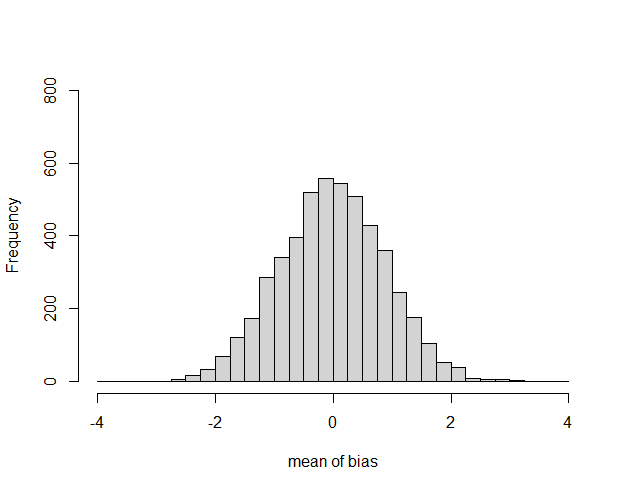
\includegraphics[scale=.5]{plots/plot4.1}
				}
				\subfigure[BLI-SPC $\rho_{partial} = 0.73$]{
					\label{boxplot:b}
					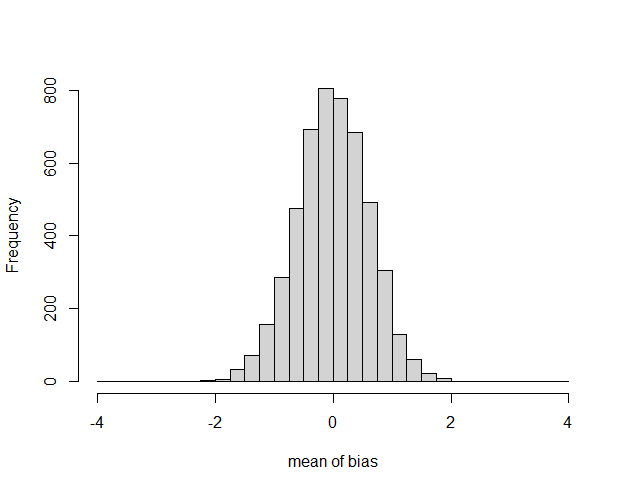
\includegraphics[scale=.5]{plots/plot4.2}
				}
			}\\ 	
			\resizebox{\textwidth}{!}{
				\subfigure[BLI-SPC $\rho_{partial} = 0.99$]{
					\label{boxplot:c}
					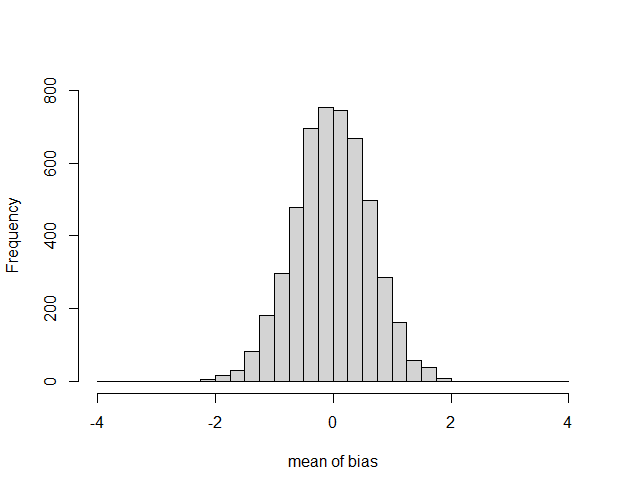
\includegraphics[scale=.5]{plots/plot4.3}
				}
				\subfigure[The targeted learning]{
					\label{boxplot:d}
					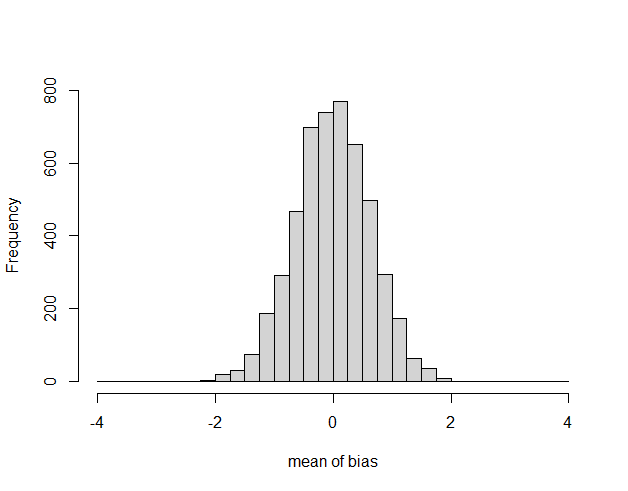
\includegraphics[scale=.5]{plots/plot4.4}
				}
			}
		\end{center}
		\caption{Histrogram plots of the mean bias for all four strategies to estimate the individual treatment effects.}
		\label{fig4_1}
	\end{figure}
	
	\begin{table}[ht!]
		\centering
		\begin{tabular}{c|cc}
			$\rho_{Y(0)Y(1)\,|\ X}$                       & Mean   & Variance \\
			\hline                              
			BLI-SPC $\rho_{partial} = 0$       & -0.012     & 0.791 \\
			BLI-SPC $\rho_{partial} = 0.73$    & -0.007     & 0.363 \\
			BLI-SPC $\rho_{partial} = 0.99$    & -0.013     & 0.398 \\
			The targeted learning         & -0.006 & 0.401 
		\end{tabular}
		\caption{The location and the scale of the mean bias for all four strategies to estimate the individual treatment effects.}
		\label{tab4_1}
	\end{table} 
	
	\begin{figure}[ht!]
		\centering
		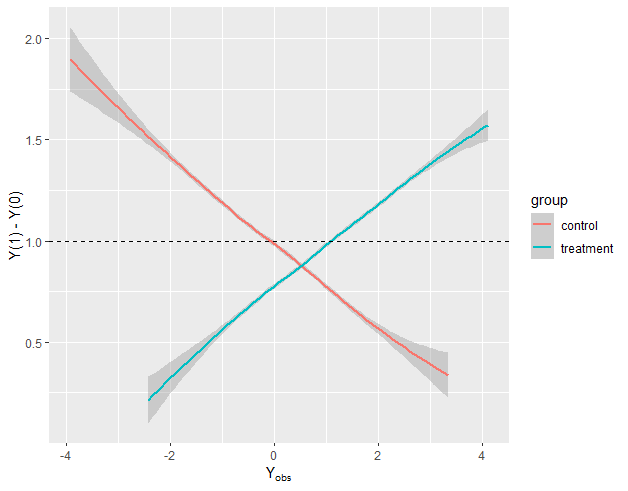
\includegraphics[width=1.0\linewidth,height=0.5\textheight]{plots/plot4.5} 
		\caption{The plot shows individual treatment effects $(Y(1) - Y(0))$ in both treatment and control group. The oucome $Y(0)$ is observed in the control group and the oucome $Y(1)$ is observed in the treatment group. The dashed line represents the average treatment effect.}
		\label{fig4_2}
	\end{figure}
	
	Overall, BLI-SPC with three different partial correlations and the targeted learning all yield unbiased estimates of the average treatment effect. However, in terms of the scale, The BLI-SPC with the ``correct" partial correlation has the smallest variance. The closer the specified partial correlation is to the ``true" value, the smaller bias and variance would be produced. When the partial correlation is specified accurately, the variance of the bias of the individual treatment effect across all cases equals the partial variance of the potential outcome. It is thus challenging to produce an accurate estimate of the individual treatment effect for a unit at the extreme. We can see this in Figure \ref{fig4_2}. However, we still have a large proportion of the estimated individual treatment effect with negligible biases. Since the variance of the bias equals the partial variance of the potential outcomes, we could include more explanatory variables to increase the accuracy of the imputation of missing outcomes and hence the prediction of individual treatment effect. On the other hand, when the specified partial correlation deviates from the ``true" value, more variance would appear because of the differences between the true distribution and the estimated distribution for each missing outcome. 
	
	
	\begin{figure}[ht!]
		\begin{center}
			\resizebox{\textwidth}{!}{
				\subfigure[BLI-SPC $\rho_{partial} = 0$]{
					\label{boxplot:e}
					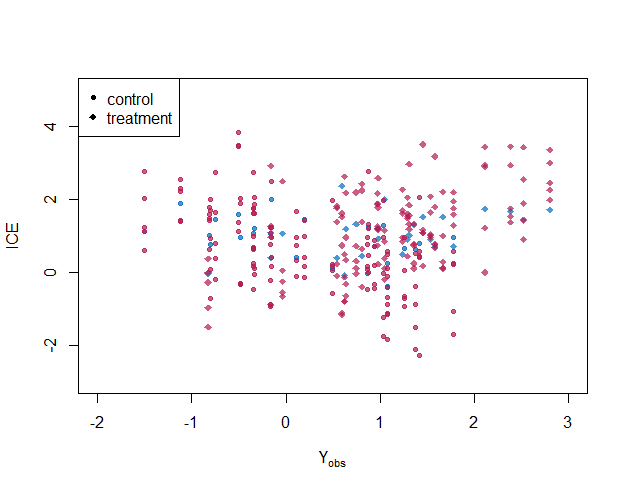
\includegraphics[scale=.5]{plots/plot4.6}
				}
				\subfigure[BLI-SPC $\rho_{partial} = 0.73$]{
					\label{boxplot:f}
					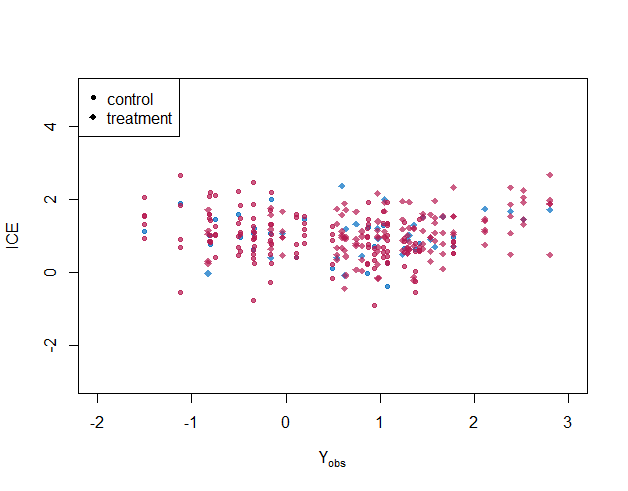
\includegraphics[scale=.5]{plots/plot4.7}
				}
			}\\ 	
			\resizebox{\textwidth}{!}{
				\subfigure[BLI-SPC $\rho_{partial} = 0.99$]{
					\label{boxplot:g}
					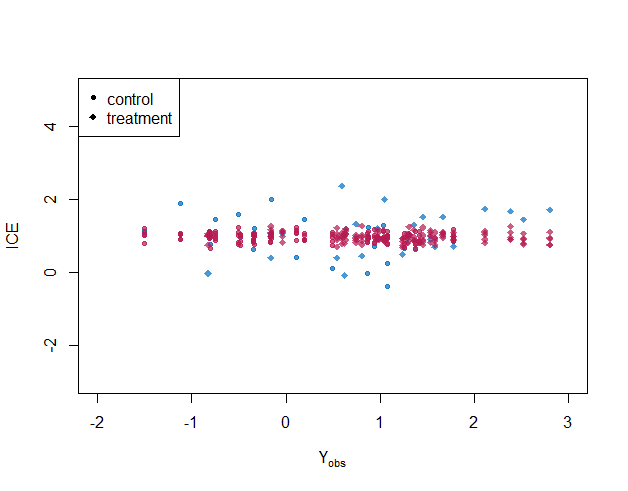
\includegraphics[scale=.5]{plots/plot4.8}
				}
				\subfigure[The targeted learning]{
					\label{boxplot:h}
					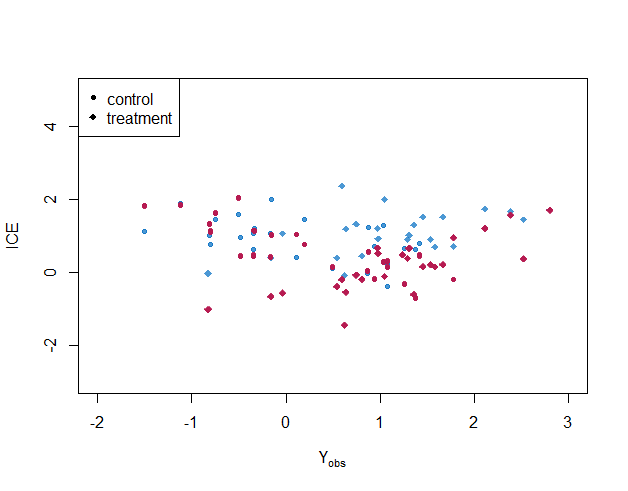
\includegraphics[scale=.5]{plots/plot4.9}
				}
			}
		\end{center}
		\caption{Stripplot of $\texttt{m} = 5$ of observed (blue) and imputed (red) data for individual treatment effects with selected cases.}
		\label{fig4_3}
	\end{figure}
	Figure \ref{fig4_3} shows individual treatment effects calculated with imputed datasets for selected cases($\emph{i} = 100, 200, \dots, 5000$). When the partial correlation is specified correctly, the imputations look plausible: imputed ICE covers the true ICE for almost every case, and the variance of ICE for each individual is smaller than the case under the independent conditional correlation assumption. With homogeneous treatment effect assumption, i.e., $\rho_{Y(0)Y(1)\,|\ X} = 0.99$, the imputed individual treatment effects are biased towards the average treatment effect. For targeted learning, uncertainty about the missing outcomes is not estimated. The BLI-SPC approach derives the distribution of individual treatment effects, which provides more information on treatment recommendations. For instance, with a small individual treatment effect, it is possible to estimate the probability of a positive causal effect from the distribution of individual treatment effect.    
	
	\subsubsection{Parameter inference}
	In this section, we investigate whether we could provide valid inferences of the distribution of the potential outcomes. The data generation mechanism follows the multivariate normal distribution introduced in section \ref{sec:4.5.1}. The simulation is repeated 1000 times. We are interested in the biases and the coverage of nominal 95\% CIs of all parameters connected to the potential outcomes.  
	\begin{table}[ht!]
		\centering
		\begin{tabular}{lccc}
			Method & Truth & Est   & Cover \\
			\hline
			BLI-SPC $\rho_{partial} = 0$       &      &      &  \\\hline
			E($y_0$)       & 0.0     & 0.00     & 0.95 \\
			E($y_1$)       & 1.0     & 1.00     & 0.94 \\
			Var($y_0$)     & 1.0     & 1.00 & 0.94 \\
			Var($y_1$)     & 1.0     & 1.00 & 0.94 \\
			Cov($y_0$, $y_1$) & 0.8   & 0.25   & 0.00 \\
			Cov($y_0$, $x$)  & 0.5   & 0.50 & 0.94 \\
			Cov($y_1$, $x$)  & 0.5   & 0.50   & 0.95\\\hline
			BLI-SPC $\rho_{partial} = 0.73$       &      &      &  \\\hline
			E($y_0$)       & 0.0     & 0.00     & 0.97 \\
			E($y_1$)       & 1.0     & 1.00     & 0.95 \\
			Var($y_0$)     & 1.0     & 1.00 & 0.94 \\
			Var($y_1$)     & 1.0     & 1.00 & 0.95 \\
			Cov($y_0$, $y_1$) & 0.8   & 0.80   & 1.00 \\
			Cov($y_0$, $x$)  & 0.5   & 0.50 & 0.95 \\
			Cov($y_1$, $x$)  & 0.5   & 0.50   & 0.94\\\hline
			BLI-SPC $\rho_{partial} = 0.99$       &      &      &  \\\hline
			E($y_0$)       & 0.0     & 0.00     & 0.95 \\
			E($y_1$)       & 1.0     & 1.00     & 0.95 \\
			Var($y_0$)     & 1.0     & 1.00 & 0.95 \\
			Var($y_1$)     & 1.0     & 1.00 & 0.94 \\
			Cov($y_0$, $y_1$) & 0.8   & 0.99   & 0.00 \\
			Cov($y_0$, $x$)  & 0.5   & 0.50 & 0.95 \\
			Cov($y_1$, $x$)  & 0.5   & 0.50   & 0.95
		\end{tabular}
		\caption{Parameter estimates for BLI-SPC with different partial correlations}
		\label{tab4_2}
	\end{table} 
	Table \ref{tab4_2} shows all statistics relevant to the potential outcomes. Statistics involving only one potential outcome are unbiased and have valid coverage rates, which means that even with incorrect specified partial correlation, we could derive plausible marginal distribution of potential outcomes. Since the partial correlation is set before imputation and there is no information about the correlation between potential outcomes in the data, we get valid inference for the marginal correlation between potential outcomes only when we specified the partial correlation correctly.  
	
	\section{Application}
	\label{sec:4.6}
	We applied our approach to evaluate the effects of two different therapies on slowing the progression of HIV disease. The data came from a study comparing the effects of four therapies (zidovudine alone, didanosine alone, zidovudine plus didanosine and zidovudine and zalcitabine) on preventing the deterioration of disease in adults with HIV-1 infected patients \citep{hammer1996trial}. For simplicity, we name them treatment A(zidovudine alone), B(didanosine alone), C(zidovudine plus didanosine) and D(zidovudine and zalcitabine). The data named ACTG175 is accessible in package speff2trial in R. We restrict our analyses to treatments A and B and perform out-of-sample prediction of hypothetical effect of treatments A and B for the remaining patients that were allocated to treatments C and D. \citet{hammer1996trial} concluded that treatment with didanosine is superior to treatment with zidovudine. However, the overall treatment effect was found to be insufficient to recommend the therapy to a patient, a situation that in common in many medical interventions. 
	
	A total of 693 HIV-1 infected adults with CD4 cell counts in the range of 200 to 500 per cubic millimeter were randomized into control (N = 316) and treatment (N = 377) group, while 670 patients are treated as out-of-sample. Fifteen baseline covariates are included which assess gender, age, weight, Karnofsky score, risk factors, prior antiretroviral therapy, CD4 cell count, and CD8 T cell count. We are interested in the number of days until the first occurrence of: 1) a decline in CD4 cell count of at least 50 2) an event indicating progression to AIDS, or 3) death. The larger number of days yields a more beneficial treatment effect. The individual treatment effect is defined as the number of days under treatment B minus the number of days under treatment A. We select the value of partial correlation as 0 and 0.7 to perform the sensitivity analysis so that the result yields distinct differences. 
	
	\begin{figure}[ht!]
		\begin{center}
			\resizebox{\textwidth}{!}{
				\subfigure[BLI-SPC $\rho_{partial} = 0$]{
					\label{boxplot:i}
					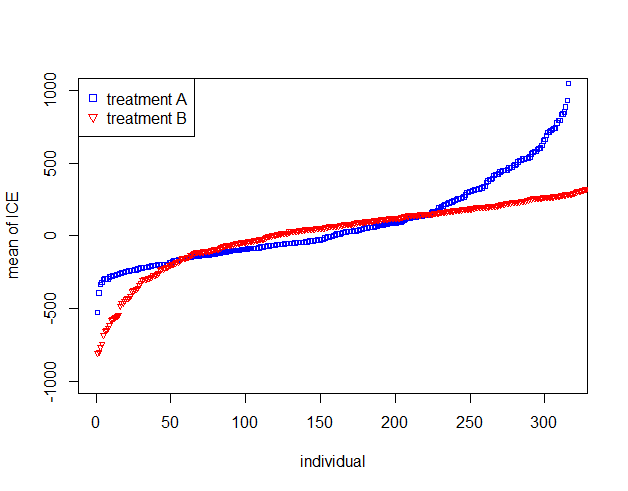
\includegraphics[scale=.5]{plots/plot4.10}
				}
				\subfigure[BLI-SPC $\rho_{partial} = 0.7$]{
					\label{boxplot:j}
					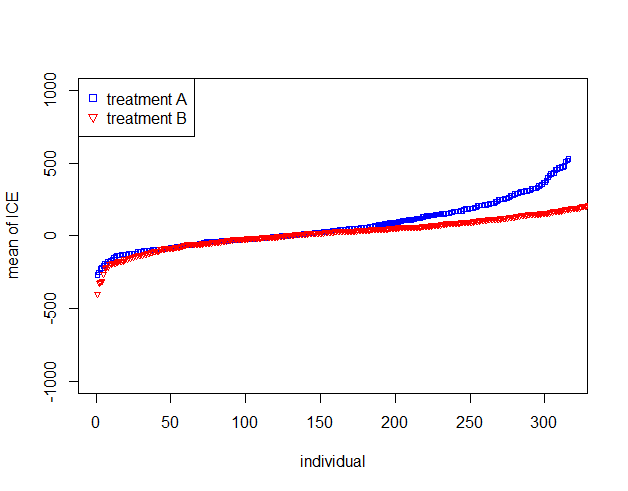
\includegraphics[scale=.5]{plots/plot4.11}
				}
			}\\
		\end{center}
		\caption{Means of individual treatment effects for patients under treatment A and treatment B, which are arranged into ascending order.}
		\label{fig4_4}
	\end{figure}
	
	\begin{figure}[ht!]
		\begin{center}
			\resizebox{\textwidth}{!}{
				\subfigure[BLI-SPC $\rho_{partial} = 0$]{
					\label{boxplot:k}
					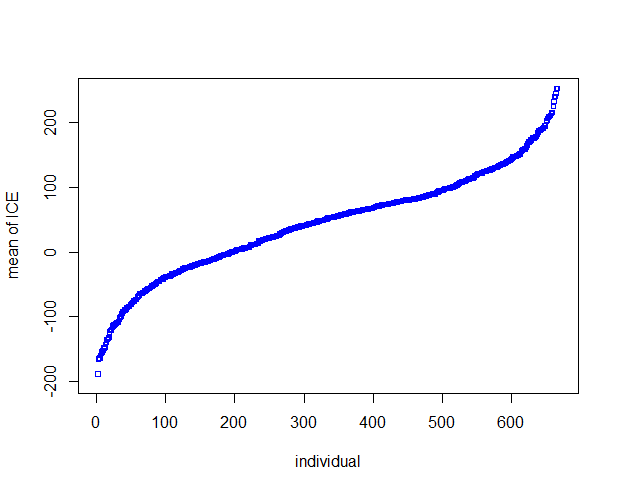
\includegraphics[scale=.5]{plots/plot4.12}
				}
				\subfigure[BLI-SPC $\rho_{partial} = 0.7$]{
					\label{boxplot:l}
					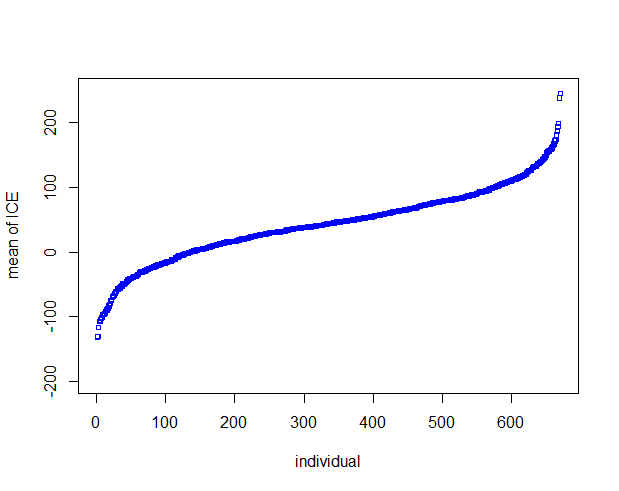
\includegraphics[scale=.5]{plots/plot4.13}
				}
			}\\
		\end{center}
		\caption{Means of individual treatment effects for out-of-sample patients under treatment C and D, which are arranged into ascending order.}
		\label{fig4_5}
	\end{figure}
	Figure \ref{fig4_4} shows the results of individual treatment effects under treatment A and treatment B group with partial correlation specification 0 and 0.7. As expected, this approach could detect the heterogeneity of treatment effects. A large proportion of patients in the sample, whose individual treatment effects are larger than 0, are recommended to receive a treatment regimen with didanosine. However, treatment with zidovudine still yields greater clinical benefit for a fraction of units, whose individual treatment effects are smaller than 0. Since all covariates are balanced under two groups, the distributions of expected individual treatment effects under two treatments (A and B) are more similar when specifying a 0.7 partial correlation. Furthermore, the range of expected value of individual treatment effects is smaller, with a partial correlation of 0.7. The larger the partial correlation we set, the more convinced that all effect modifiers are included, and effects are identical across persons. Figure \ref{fig4_5} shows variability in individual effects in out-of-sample patients, which implies that our method could also be applied to prediction. 
	\begin{figure}[ht!]
		\begin{center}
			\resizebox{\textwidth}{!}{
				\subfigure[]{
					\label{boxplot:m}
					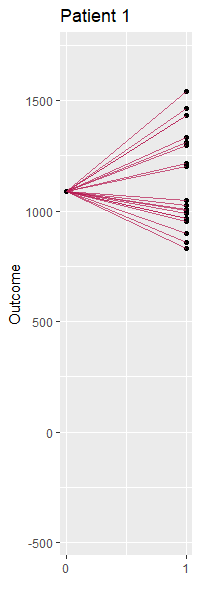
\includegraphics[scale=.5]{plots/indiv01}
				}
				\subfigure[]{
					\label{boxplot:n}
					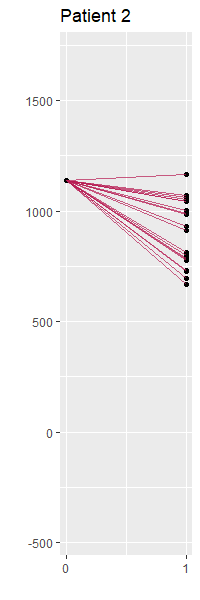
\includegraphics[scale=.5]{plots/indiv02}
				}
				\subfigure[]{
					\label{boxplot:o}
					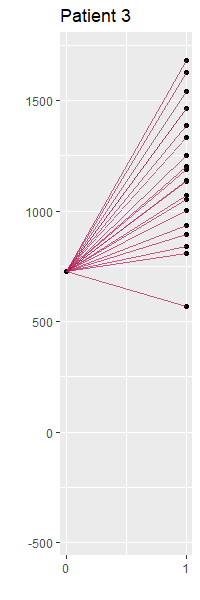
\includegraphics[scale=.5]{plots/indiv03}
				}
				\subfigure[]{
					\label{boxplot:p}
					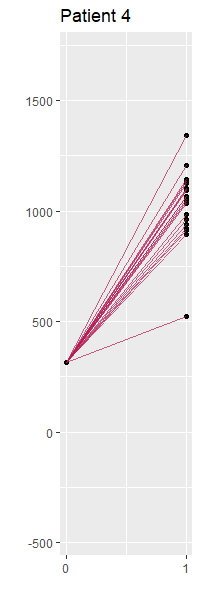
\includegraphics[scale=.5]{plots/indiv04}
				}
				\subfigure[]{
					\label{boxplot:q}
					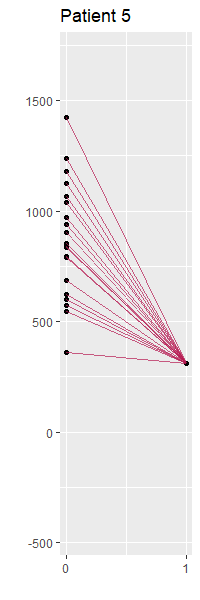
\includegraphics[scale=.5]{plots/indiv05}
				}
				\subfigure[]{
					\label{boxplot:r}
					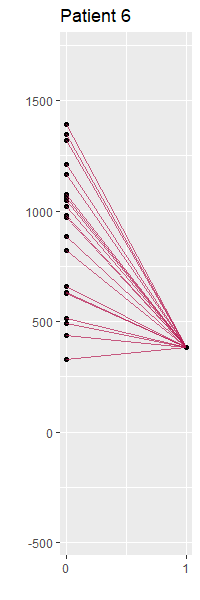
\includegraphics[scale=.5]{plots/indiv06}
				}
				\subfigure[]{
					\label{boxplot:s}
					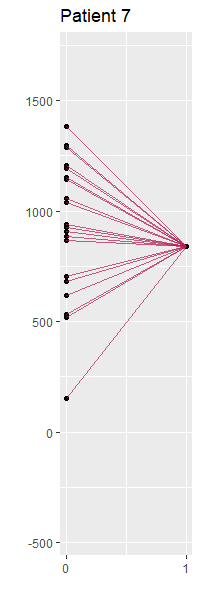
\includegraphics[scale=.5]{plots/indiv07}
				}
			}\\
		\end{center}
		\caption{Fan plot of Observed and imputed (m = 20) outcomes under treatment A (0) and B (0). The partial correlation is 0.}
		\label{fig4_6}
	\end{figure}
	
	\begin{figure}[ht!]
		\begin{center}
			\resizebox{\textwidth}{!}{
				\subfigure[]{
					\label{boxplot:t}
					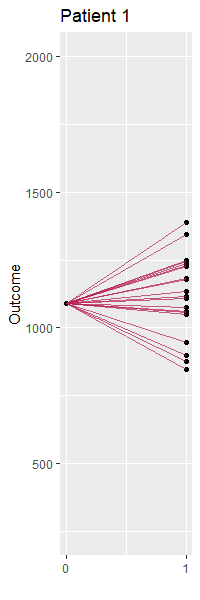
\includegraphics[scale=.5]{plots/indiv71}
				}
				\subfigure[]{
					\label{boxplot:u}
					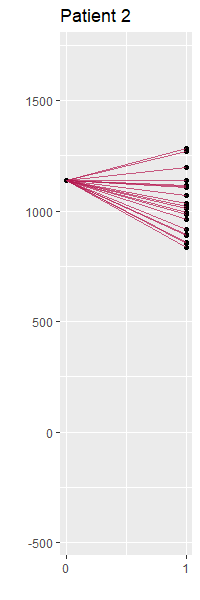
\includegraphics[scale=.5]{plots/indiv72}
				}
				\subfigure[]{
					\label{boxplot:v}
					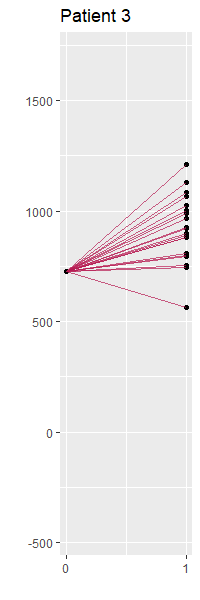
\includegraphics[scale=.5]{plots/indiv73}
				}
				\subfigure[]{
					\label{boxplot:w}
					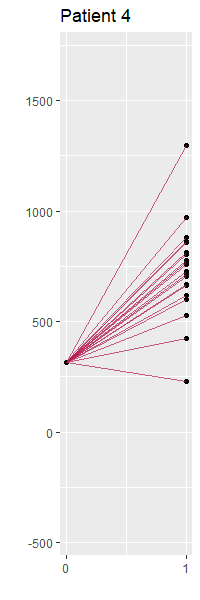
\includegraphics[scale=.5]{plots/indiv74}
				}
				\subfigure[]{
					\label{boxplot:x}
					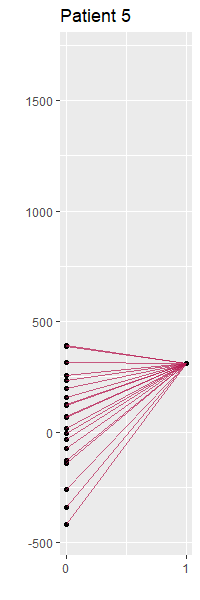
\includegraphics[scale=.5]{plots/indiv75}
				}
				\subfigure[]{
					\label{boxplot:y}
					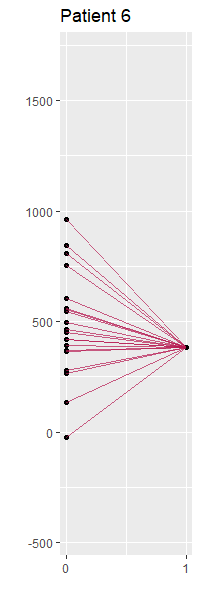
\includegraphics[scale=.5]{plots/indiv76}
				}
				\subfigure[]{
					\label{boxplot:z}
					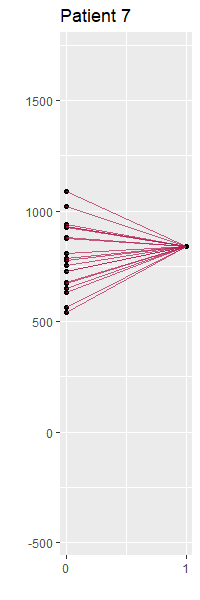
\includegraphics[scale=.5]{plots/indiv77}
				}
			}\\
		\end{center}
		\caption{Fan plot of Observed and imputed (m = 20) outcomes under treatment A (0) and B (0). The partial correlation is 0.7.}
		\label{fig4_7}
	\end{figure}
	Figure \ref{fig4_6} and \ref{fig4_7} display imputations by selected patients for two different values of partial correlation, 0 and 0.7. Each panel contains the observed outcome for the patient and $m = 20$ imputed values for the missing outcome. The imputed outcomes are sensitive to different values of partial correlation. Patient 5 benefits from treatment A when the partial correlation equals 0, while we derive the opposite conclusion when specifying the partial correlation as 0.7. The location of imputed outcomes is different under various partial correlations, and the scale shrinks when the partial correlation tends to 1.  
	
	\section{Discussion}
	\label{sec:4.7}
	Treatment assignment is currently steered by the average treatment effect. This may lead to the suboptimal individual treatment decision when the assumption of homogeneous treatment effect is not true. More often than not, we lack the explanatory variables that would render the ATE homogeneous. This paper proposes a multiple imputation approach to replace missing outcomes with plausible values to estimate the individual treatment effect. Our method allows researchers to consider the correlation between potential outcomes, which influence the imputation of missing outcomes.  
	
	The sensitivity analysis of the partial correlation between potential outcomes in section \ref{sec:4.5.3}  demonstrates that different values of the partial correlation yielded similar results in terms of marginal distributions of potential outcomes and the average treatment effect. However, the closer the specified partial correlation is to the ``true" value, the less biased the estimated individual treatment effect will be. Since one cannot obtain information about the partial correlation from the observed data, the determination of the partial correlation should be set to a plausible range based on previous investigations or expert knowledge. In addition, it may be useful to perform a sensitivity analysis to see how imputed outcomes differ with different partial correlations. 
	
	An advantage of our multiple imputation approach to individual treatment effects is that it provides an estimate of the uncertainty of the imputed outcomes and hence, of the individual treatment effects. One could obtain the posterior distribution of the individual treatment effects for a unit from multiply imputed datasets, from which we can learn the probability of benefit from the treatment at the individual level. Since we incorporate the partial correlation when imputing, researchers could apply complete-data analyses to explore potential variables. This is accounting for residual heterogeneity of treatment effects or additional effect modifiers. 
	
	In our illustration of the BLI-SPC algorithm, we applied Bayesian imputation under the normal linear model. It is possible to use other imputation techniques (parametric or non-parametric imputation methods). The behavior of such methods have not yet been studied. Another useful property of BLI-SPC is that under the assumption of ignorable treatment assignment, researchers can skip explicit modeling of the probability of assignment. The BLI-SPC is a hybrid of FCS and JM, and hence it also provides valid imputations with MAR. 
	
	In the application study, we focus on the comparison of treatments A and B. It is possible to generalize to the multiple treatment comparison (treatment A, B, C, and D). By imputing unobserved outcomes, we could recommend the optimal treatment to each unit among four treatments. One could benefit from our method when performing an experiment that has been investigated on a different population. Some proven effect modifiers may be difficult to collect when performing the same experiment in other regions or countries. In such a case, the inference would include the heterogeneity of treatment effects explained by the uncollected factors by specifying a reasonable partial correlation.         
	
	This is an initial study on MI to the individual treatment effect. The simulation study used a basic randomized trial with a correctly specified imputation model. Further work should be done to extend discrete and semi-continuous outcomes. Another challenge is to develop imputation techniques for studies that collect post-treatment variables. All in all, we believe that our methodology for incorporating the partial correlation represents an important advance in estimating individual treatment effects. We hope that our method may attribute to put down the shackles of the ubiquitous average treatment effect.  
